\documentclass{beamer}

\usepackage[pantone315,english]{wwustyle}

\usepackage{etoolbox}
\usepackage[ngerman]{babel}
\usepackage[utf8]{inputenc}
\usepackage[T1]{fontenc}
\usepackage{xspace}

\definecolor{dkgreen}{rgb}{0,0.6,0}
\definecolor{mauve}{RGB}{127,0,85}

\usetikzlibrary{calc,fit,matrix,shapes,positioning,shadows,arrows,decorations.text}
\tikzstyle{every picture}+=[remember picture]

\tikzset{
	invisible/.style={opacity=0},
	visible/.style={alt=#1{}{invisible}},
	alt/.code args={<#1>#2#3}{%
		\alt<#1>{\pgfkeysalso{#2}}{\pgfkeysalso{#3}}
	},
	highlight/.style={maincolor, alt=#1{}{plain}},
	plain/.style={pantoneblack7},
}

\pgfdeclarelayer{bg}    % declare background layer
\pgfdeclarelayer{fg}    % declare foreground layer
\pgfsetlayers{bg,main,fg}  % set the order of the layers (main is the standard layer)



% SOURCE CODE FORMATTING
\usepackage{listings}
\lstdefinelanguage{MD2}{
  morekeywords={@Check, @Test, MD2Package, ControllerValidator, def, assertError,  WorkflowElement,processChain,invokable,using,at,WorkflowElements, fires, start, App, startable, appName, package, entity, string,
  date, float, enum, integer, boolean, time, datetime, GridLayoutPane, FlowLayoutPane, TabbedPane, TextInput,
  label, tooltip, type, default, timestamp, OptionInput, options, CheckBox, checked, Label, text, style, Tooltip,
  Button, Image, height, width, src, Spacer, AutoGenerator, exclude, only, textProposition, contentProvider,
  ContentProvider, EntitySelector, color, fontSize, textStyle, main, appVersion, modelVersion, workflowManager,
  defaultConnection, CustomAction, CombinedAction, CustomCodeFragement, SimpleAction, WebServiceCallAction, WebServiceCall, externalWebService, url, method, GET, POST, PUT, DELETE, queryparams, bodyparams, on, from, Container, Content,
  GlobalEventType, OnConditionEvent, elementEventType, GotoViewAction, Workflow, WorkflowStep, ContentProvider, use,
  for, to, latitude, longitude, altitude, citystreet, number, postalCode, country, province, ElementEventType, event,
  valid, empty, filled, and, equals, not, is, or, Condition, Boolean, bind, unbind, Validator, ContainerElement,
  ContentElement, validator, IsIntValidator, NotNullValidator, IsNumberValidator, IsDateValidator, RegExValidator,
  NumberRangeValidator, StringRangeValidator, map, unmap, call, actions, message, min, max, regEx, format, minLength,
  maxLength, RemoteValidator, connection, model, attributes, workflow, ProcessChainStep,step, view, forwardCondition,
  forwardMessage, backwardMessage, backwardCondition, forwardOnEvent, backwardOnEvent, forwardEvents, subProcessChain,
  remoteConnection, uri, ProcessChain, end, defaultProcessChain, onInit, FireEvent, ProcessChainProceed, ProcessChainReverse, ProcessChainGoto, SetProcessChain, GotoView, where, Location, Disable, Enable, DisplayMessage, ContentProviderOperation, ContentProviderReset, inputs, outputs, cityInput, streetInput, streetNumberInput, postalInput, countryInput,FileUpload, UploadedImageOutput, imgHeight,imgWidth,fileUploadConnection, storagePath, file, optional,
  latitudeOutput, longitudeOutput, name, description, proceed, reverse, goto, return, given, do, returnTo, disabled,
  action, if, else, set, elseif},
  otherkeywords={},
  sensitive=true,
  morecomment=[l]{//},
  morecomment=[n]{/*}{*/},
  morestring=[b]",
  morestring=[b]',
  morestring=[b]"""
}
\lstset{
  language=MD2,
  aboveskip=3mm,
  belowskip=3mm,
  showstringspaces=false,
  columns=flexible,
  basicstyle={\scriptsize\ttfamily},
  numbers=none,
  numberstyle=\tiny\color{gray},
  keywordstyle=\color{pantone315},
  commentstyle=\color{dkgreen},
  stringstyle=\color{pantone390},
  breaklines=true,
  breakatwhitespace=true
  tabsize=3
}
% END SOURCE CODE FORMATTING

\usepackage{setspace}

%---------------------------------------------------------------------
%% Navigation Bar
\setbeamertemplate{footline}{
  \fontsize{6pt}{1pt}
  \selectfont
  \vskip4pt
  \color{maincolor}
  \rule{\textwidth}{1.2pt}\\ % horizontal line
  \vskip2pt
  \rule{\textwidth}{0.8pt}\\ % horizontal line
  \vskip5pt
  \rule{\textwidth}{1.2pt} % horizontal line
  \vskip2pt
  \color{black}
  \hspace{5.1mm}
  \insertshortauthor 
  \begin{beamercolorbox}[ht=0cm, leftskip=3ex]{section in head/foot}
    \insertsectionnavigationhorizontal{.75\paperwidth}{}{}
  \end{beamercolorbox}
  \vskip1.8pt
}

%% Automatic Outline
\AtBeginSection[]
{
	\ifnumequal{\value{framenumber}}{1}{%
	\begin{frame}{Outline}
		\tableofcontents[currentsection, sectionstyle=show/show, subsectionstyle=hide/hide/hide, subsubsectionstyle=hide/hide/hide]
	\end{frame}
	\addtocounter{framenumber}{-1}
	}{}

	\begin{frame}{Outline}
		\tableofcontents[currentsection, sectionstyle=show/shaded, subsectionstyle=hide/hide/hide, subsubsectionstyle=hide/hide/hide]
	\end{frame}
}
%% Numbered and Colored TOC
\setbeamertemplate{section in toc}{\leavevmode\usebeamercolor[fg]{section in toc}\inserttocsectionnumber. \usebeamercolor[fg]{normal text}\inserttocsection\par}
\setbeamertemplate{subsection in toc}{\leavevmode\leftskip=1em\usebeamercolor[fg]{section in toc}\inserttocsectionnumber.\inserttocsubsectionnumber\, \usebeamercolor[fg]{normal text}\inserttocsubsection\par}

%---------------------------------------------------------------------


%Show page number on plain frames with command \plainnumber
\newcommand{\plainnumber}{%
\begin{tikzpicture}[remember picture, overlay]
    \node at ($(current page.north east)+(-.3,-.3)$)[anchor= north east]{ %
      \tiny{\insertframenumber{}} };
\end{tikzpicture}
}

\newcommand{\MD}{MD$^2$\xspace}
\newcommand{\mapapps}{map.apps\xspace}
\newcommand{\codeheading}[1]{
	{\small{}#1\\[-1.5ex]
	\color{gray}\rule{\linewidth}{0.4pt}}\\[-1ex]
}
\newcommand{\quelle}[1]{{\tiny{\color{gray}{\,#1}}}}

%---------------------------------------------------------------------

\author{Project Seminar \MD}
\title{Model-Driven Mobile Development}
%\institutelogo{Logo on title frame}
%\institutelogosmall{Logo on other frames}
\subtitle{\MD for map.apps}


\begin{document}

	\begin{frame}[plain]
	  \maketitle
	\end{frame}
    
    \section{Motivation}
    \begin{frame}[t]
    \frametitle{Why MD2?}
    
    \begin{itemize}
       \item Cross-Platform approach
       \item Develop a model once, for multiple mobile platforms
       \item Decrease maintenance costs
       \item bla blub bla
    \end{itemize}
\end{frame}

\begin{frame}[t]
    \frametitle{Starting base of MD2}
    
    \begin{center}   
	    \begin{tikzpicture}
		    \draw [fill=gray!30!white] (-4,5) rectangle (4,5.5) node[pos=.5] {MD2 Model};
		    \draw [fill=gray!10!white] (-4,4.5) rectangle (-1.3,5) node[pos=.5] {Model};
		    \draw [fill=gray!10!white] (-1.3,4.5) rectangle (1.3,5) node[pos=.5] {View};
		    \draw [fill=gray!10!white] (1.3,4.5) rectangle (4,5) node[pos=.5] {Controller};
		    
		    \draw [->] (0,4.5) -- (0,4.3);
		    
		    \draw [fill=gray!30!white] (-4,3.8) rectangle (4,4.3) node[pos=.5] {Preprocessing};
		    
		    \draw [->] (0,3.8) -- (0,3.6);
		    
		    \draw [fill=gray!30!white] (-4,3.1) rectangle (4,3.6) node[pos=.5] {Completed MD2 Model};
		    
		    \draw [->] (0,3.1) -- (-2,2.8);
		    \draw [->] (0,3.1) -- (0,2.8);
		    \draw [->] (0,3.1) -- (2,2.8);
		    
		    \draw [gray!30!white, dashed] (-5.5,3) rectangle (5.5,2.2);
		    \node [right] at (-5.5,2.8) {\scriptsize{\textit{Code}}};
		    \node [right] at (-5.5,2.5) {\scriptsize{\textit{Generators}}};
		    		    
		    \draw [fill=gray!30!white] (-4,2.3) rectangle (-1.5,2.8) node[pos=.5] {Android};
		    \draw [fill=gray!30!white] (-1.3,2.3) rectangle (1.3,2.8) node[pos=.5] {Backend};
		    \draw [fill=gray!30!white] (1.5,2.3) rectangle (4,2.8) node[pos=.5] {iOS};
		    
		    \draw [->] (-2.75,2.3) -- (-2.75,2);
		    \draw [->] (0,2.3) -- (0,2);
		    \draw [->] (2.75,2.3) -- (2.75,2);
		    
		    \draw [fill=gray!30!white] (-4,1.5) rectangle (-1.5,2) node[pos=.5] {Source code};
		    \draw [fill=gray!30!white] (-1.3,1.5) rectangle (1.3,2) node[pos=.5] {Source code};
		    \draw [fill=gray!30!white] (1.5,1.5) rectangle (4,2) node[pos=.5] {Source code};
		    
		    \draw [->] (-2.75,1.5) -- (-2.75,1.2);
		    \draw [->] (0,1.5) -- (0,1.2);
		    \draw [->] (2.75,1.5) -- (2.75,1.2);
		    
		    \draw [fill=gray!30!white] (-4,0.7) rectangle (-1.5,1.2) node[pos=.5] {Android app};
		    \draw [fill=gray!30!white] (-1.3,0.7) rectangle (1.3,1.2) node[pos=.5] {Container};
		    \draw [fill=gray!30!white] (1.5,0.7) rectangle (4,1.2) node[pos=.5] {iOS app};	
		    
		    \draw [<->] (-1.5,0.95) -- (-1.3,0.95); 
		    \draw [<->] (1.5,0.95) -- (1.3,0.95);    
		    
	    \end{tikzpicture}
    \end{center}
    
{\color{gray}{\tiny{Source: MD2 Project Seminar Presentation}}}

\end{frame}



\begin{frame}[t]
    \frametitle{Project Goals}
    
    \begin{itemize}
       \item Implement and extend generator for map.apps platform
       \item bla blub bla
    \end{itemize}
\end{frame}



    
    \section[Features]{New Features and Implementation}
    % !TEX root = ../beamer.tex

\begin{frame}[fragile, plain]
	\plainnumber
	\frametitle{Workflow Specification}
	
	\begin{minipage}{0.45\textwidth}
	    		        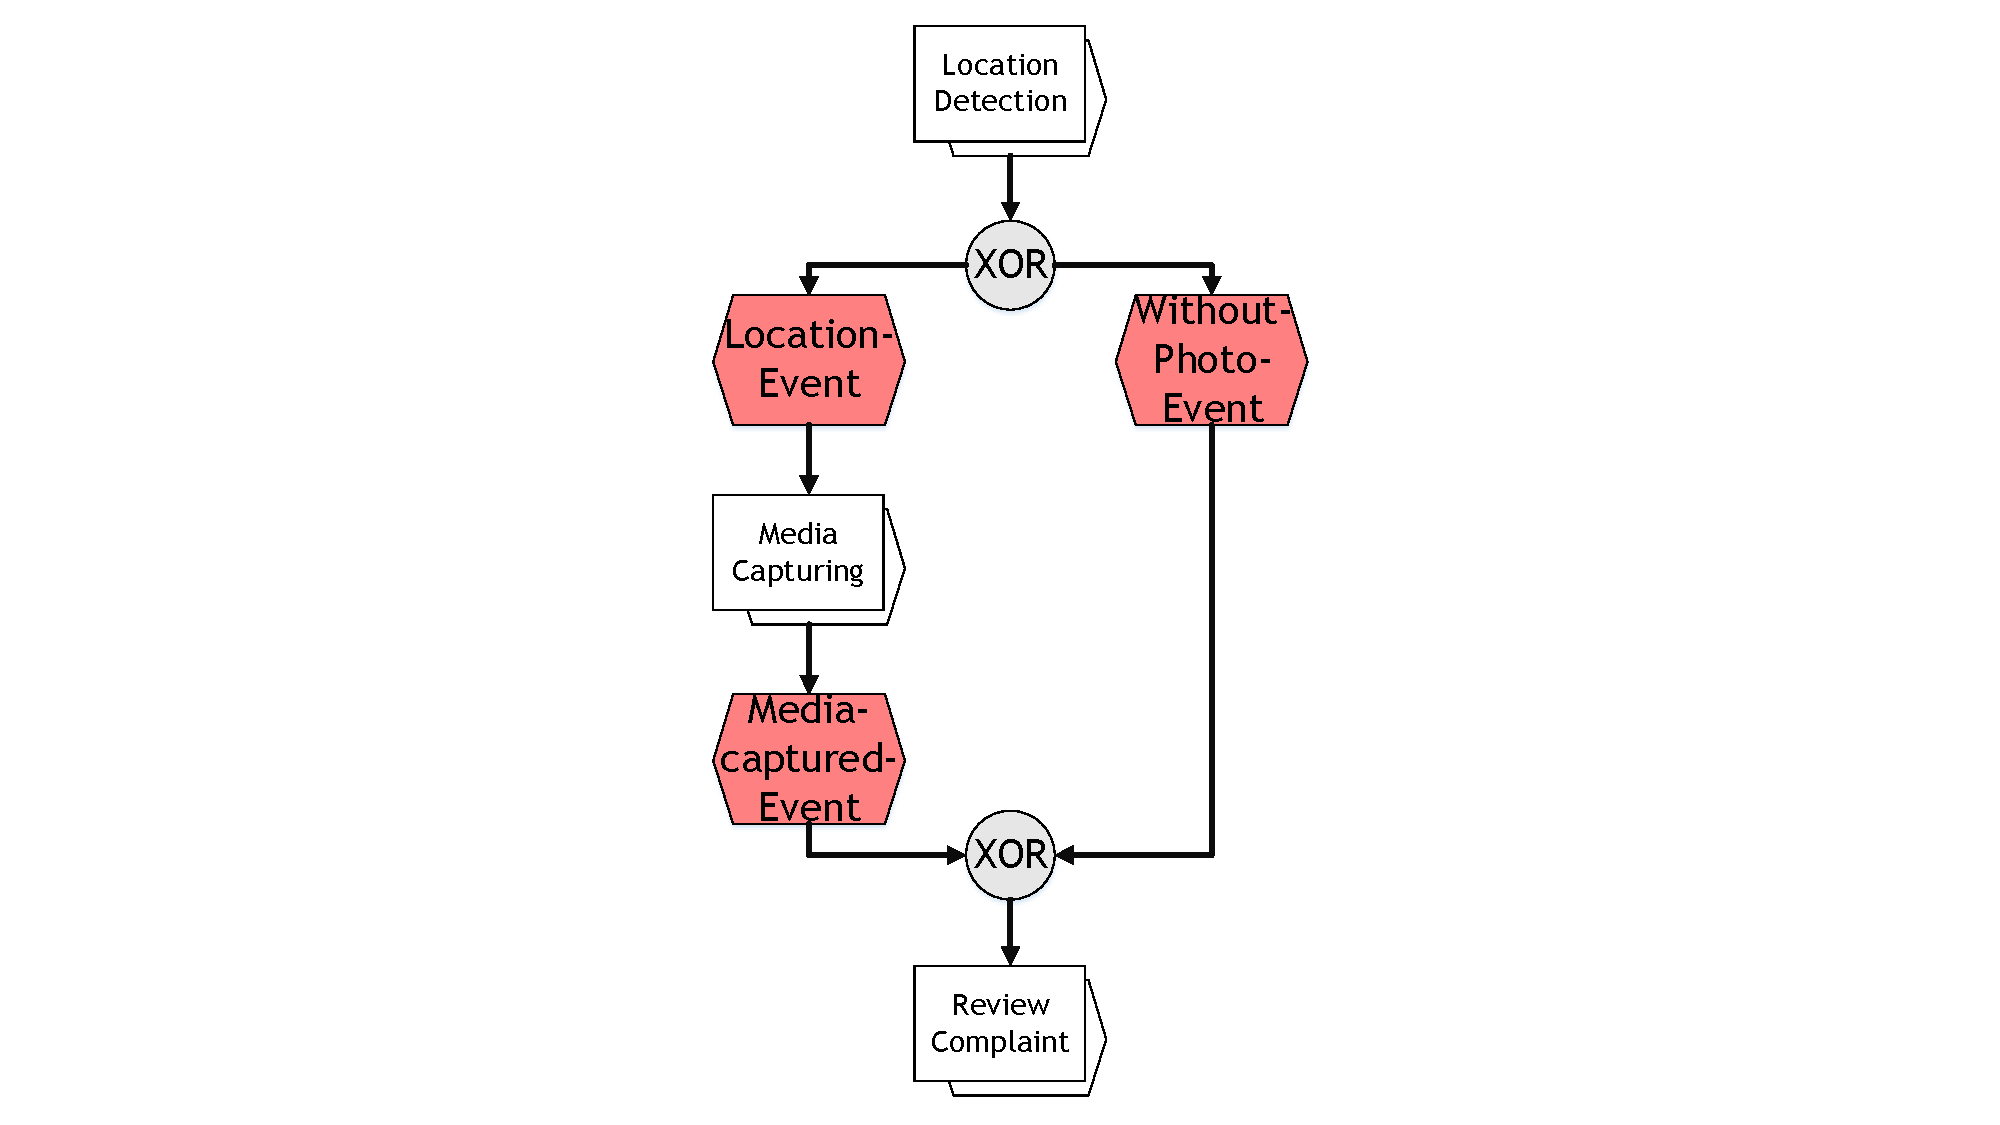
\includegraphics[height = 7cm, trim = 10cm 0cm 10cm 0cm, clip = true]{images/WorkflowSpecification.pdf}	  
	\end{minipage}\hfill
	\begin{minipage}{0.5\textwidth}
\begin{lstlisting}
WorkflowElement LocationDetection
  fires LocationEvent {
    start Mediacapturing
  }
  fires WithoutPhotoEvent {
    start ReviewComplaint
  }

WorkflowElement MediaCapturing
  fires MediacapturedEvent {
    start ReviewComplaint
  }

WorkflowElement ReviewComplaint
  fires EndEvent {
    end workflow
  }
\end{lstlisting}
\end{minipage}

\end{frame}

\begin{frame}[fragile]
 \frametitle{Workflow Element Specification, Controller Layer}
 
\begin{lstlisting}
main {
	appVersion "1.0" 
	modelVersion "1.0"
	...
}

WorkflowElement LocationDetection{
	defaultProcessChain LocationProcessChain
	onInit {
		init,
		...
	}	
	action CustomAction init{
		bind action FireEvent(LocationEvent) on LocationVerifyView.Next.onClick
		bind action FireEvent(WithoutPhotoEvent) on LocationVerifyView.SkipUpload.onClick
	}
}
\end{lstlisting}
\end{frame}

%-----------------------------------------------------------------------------------

\begin{frame}[fragile, plain]
	\plainnumber
	\frametitle{Workflow Specification Across Apps}
	
	\begin{minipage}{0.45\textwidth}
	    		        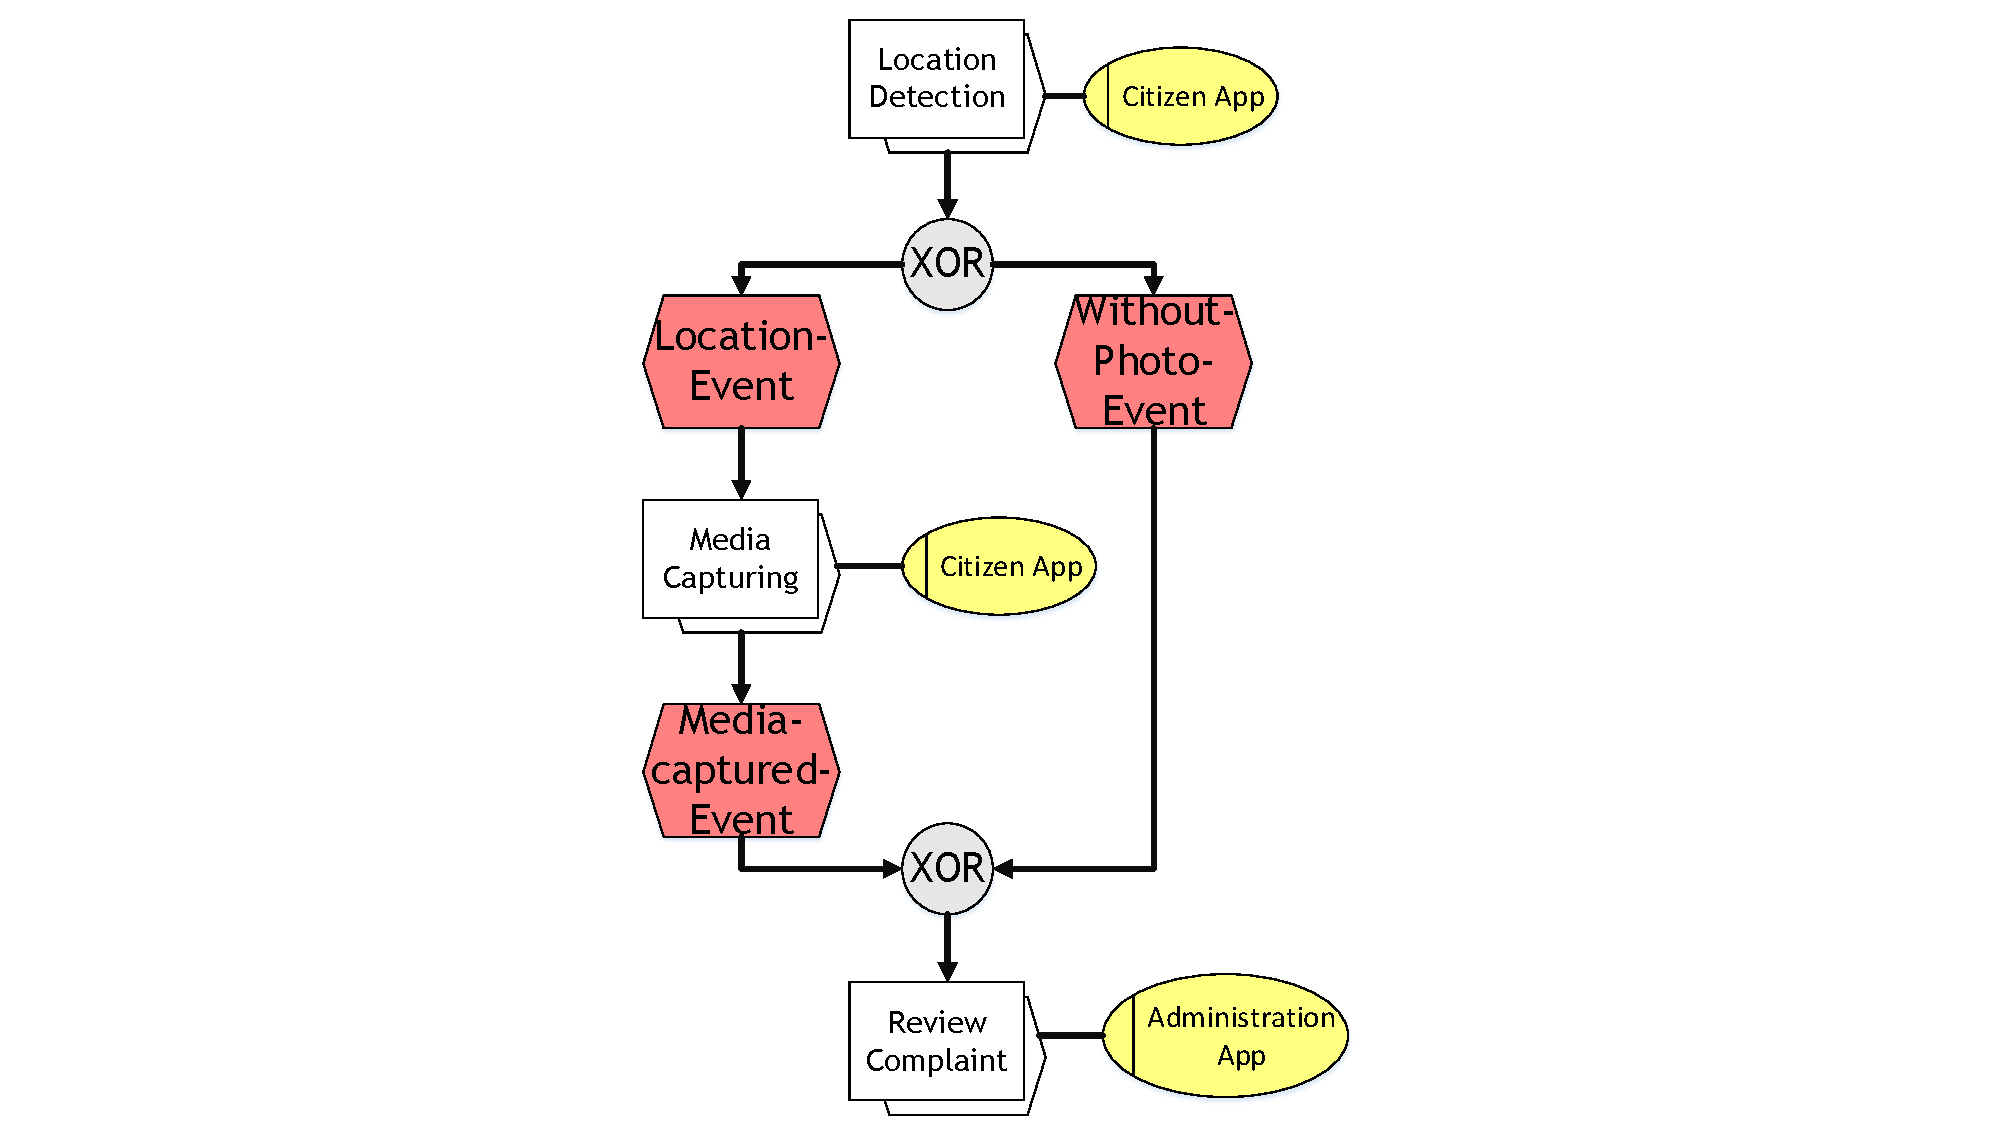
\includegraphics[height = 7cm, trim = 10cm 0cm 10cm 0cm, clip = true]{images/wfAcrossApps}	  
	\end{minipage}\hfill
	\begin{minipage}{0.5\textwidth}
\begin{lstlisting}
App CitizenApp {
  WorkflowElements {
    LocationDetection (startable: "Start Complaint"),
    MediaCapturing
  }
}

App AdministrationApp {
  WorkflowElements {
    ReviewComplaint
  }
}
\end{lstlisting}
\end{minipage}

\end{frame}

%-----------------------------------------------------------------------------------

\begin{frame}[plain]

\plainnumber

\frametitle{Implementation: WorkflowEventHandler}

\begin{center}
	\begin{tikzpicture}[
	>=stealth,
	wfe/.style = {draw, circle, fill=black!15!white},
	eh/.style = {draw, minimum height = 3cm, minimum width = 3cm, fill=pantone315!30!white}
	]
		\node (citizen) {
\includegraphics[width=0.5cm]{images/stickfigure}};
		\node[below = 0cm of citizen] (citizenlbl) {\scriptsize Citizen};
		
		\node[wfe, below = of citizenlbl] (wfe1) {WFE1};
		\node[wfe, below = of wfe1] (wfe2) {WFE2};
		\node[eh, right = 2cm of wfe1.north east, anchor = north west] (eh) {Event Handler};
		\node[draw, minimum width = 2cm, minimum height = 1cm, right = 2cm of eh, fill=pantone369!20!white] (be) {Backend};
		
		\begin{pgfonlayer}{bg}
			\draw[fill=pantone396!10!white, draw=pantone396] ($ (wfe1.north west) + (-0.4, 0.4) $) rectangle  ($ (eh.south east) + (0.5, -0.5) $);
		\end{pgfonlayer}
		
		\draw[->, thick, visible=<1->] (citizenlbl) -- node[right] {\scriptsize{\texttt{start}}} (wfe1);
		\draw[->, thick, visible=<2->] (wfe1) -- node[above, sloped] {\scriptsize{\texttt{wfe1, event}}} (eh);
		\draw[->, thick, visible=<3->] (eh.west) -- node[above, sloped] {\scriptsize{\texttt{changeWFE}}} (wfe2.north east);
		\draw[->, thick, visible=<4->] (wfe2.east) -- node[below, sloped] {\scriptsize{\texttt{wfe2, event}}} (eh);
		\draw[->, thick, visible=<5->] (eh) -- node[above] {\scriptsize{\texttt{wfe2, event}}} (be);
		
		\visible<6->{
			\node[above right = 0.75cm and 1.5cm of citizenlbl] (admin) {
\includegraphics[width=0.5cm]{images/stickfigure}};
			\node[below = 0cm of admin] (adminlbl) {\scriptsize Admin};
			\node[draw, fill=black!15!white, right = of admin, minimum width = 2cm, minimum height = 1cm] (looi) {LOOI};
			
			\draw[->, thick] (admin) -- node[above] {\scriptsize{\texttt{show}}} (looi);	
		}
		\visible<7>{
			\node[overlay, align=center,right = 0.5cm of looi, rectangle callout, drop shadow, fill=white, draw, minimum width = 2.5cm, minimum height = 1.5cm, callout absolute pointer = {(looi)}] (popup) {
				\begin{tikzpicture}
				{\tikzset{wtf/.style = {rectangle, draw=none, fill=none, minimum width = 0cm, minimum height = 0cm }}
					\draw (0,0) -- (2, 0);
					\draw (0.5, 0.25) -- ++(0, -1.25);
					\draw (1.25, 0.25) -- ++(0, -1.25);
					\node[wtf]  at (0, 0.15) {\tiny\texttt{ID}};
					\node[wtf] at (0.5, 0.15) {\tiny\texttt{WFE}};
					\node[wtf] at (1.25, 0.15) {\tiny\texttt{\dots}};
					\node[wtf] at (0, -0.3) {\tiny\texttt{01}};
					\node[wtf] at (0.5, -0.3) {\tiny\texttt{WFE1}};
					\node[wtf] at (1.25, -0.3) {\tiny\texttt{\dots}};
					\node[wtf] at (0, -0.6) {\tiny\texttt{02}};
					\node[wtf] at (0.5, -0.6) {\tiny\texttt{WFE3}};
					\node[wtf] at (1.25, -0.6) {\tiny\texttt{\dots}};
					\node[wtf] at (0, -0.9) {\tiny\texttt{03}};
					\node[wtf] at (0.5, -0.9) {\tiny\texttt{\dots}};
					\node[wtf] at (1.25, -0.9) {\tiny\texttt{\dots}};
					}
				\end{tikzpicture}
			};
		}
		\draw[->, thick, visible=<8->] ($(looi.east) + (0, 0.1) $) -| node[right] {\scriptsize{\texttt{appID}}} ($(be.north) + (0.1, 0)$);
		\draw[<-, thick, visible=<9->] ($(looi.east) + (0, -0.1) $) -| node[below left] {\scriptsize{\texttt{open issues}}} ($(be.north) + (-0.1, 0)$);
		\visible<10->{
			\node[wfe, below right = 0.5cm of looi] (wfe3) {WFE3};
			\draw[->, thick] (looi) |- node[above right] {\scriptsize{\texttt{start}}} (wfe3);	
		}
		\begin{pgfonlayer}{bg}
			\draw[fill=pantone396!10!white, draw=pantone396, visible=<6->] ($ (looi.north west) + (-0.4, 0.4) $) rectangle  ($ (wfe3.south east) + (0.5, -0.5) $);
		\end{pgfonlayer}		
	\end{tikzpicture}
\end{center}

\end{frame}

%-----------------------------------------------------------------------------------

\begin{frame}
    \frametitle{map.apps Architecture}
	\begin{center}
	\begin{tikzpicture}[
		>=stealth,
		box/.style = {draw, minimum width = 3cm, minimum height = 1.5em, outer sep=0},
		box2/.style = {box, minimum width = 3.5cm},
		node distance = 0.1cm
		]
		
		\node[box, fill=pantone315!10!white] (wfe1) {WfE 1};
		\node[box, right = of wfe1, fill=pantone315!10!white] (wfe2) {WfE 2};
		\node[box, minimum width=6.1cm, below = of wfe1.south west, anchor = north west, fill=pantone315!10!white] (wfEventHandler1) {WorkflowEventHandler};
		\node[box, below = of wfEventHandler1.south west, anchor=north west, fill=pantone315!10!white] (models1) {Models};
		\node[box, right = of models1, fill=pantone315!10!white] (contentProv1) {ContentProvider};
		\draw ($(wfe1.north west) + (-0.1, 0.6)$) node[below right] {\textbf{App 1}} rectangle ($(contentProv1.south east) + (0.1, -0.1)$);
		
		\node[box, below = 2.3cm of wfe1, fill=pantone315!10!white] (wfe3) {WfE 3};
		\node[box, below = 2.3cm of wfe2, fill=pantone315!10!white] (wfe4) {WfE 4};
		\node[box, below = of wfe3.south west, anchor = north west, minimum width=6.1cm, fill=pantone315!10!white] (wfEventHandler2) {WorkflowEventHandler};
		\node[box, below = of wfEventHandler2.south west, anchor=north west, fill=pantone315!10!white] (models2) {Models};
		\node[box, right = of models2, fill=pantone315!10!white] (contentProv2) {ContentProvider};
		\draw ($(wfe3.north west) + (-0.1, 0.6)$) node[below right] {\textbf{App 2}} rectangle ($(contentProv2.south east) + (0.1, -0.1)$);
		
		\draw[<->, thick] ($ (wfEventHandler1.east) + (0.1, 0) $) -- ++(0.8,0);
		\draw[<->, thick] ($ (wfEventHandler2.east) + (0.1, 0) $) -- ++(0.8,0);
		
		\node[box2, right = 1cm of wfe2.north east, anchor=north west, fill=pantone315!10!white]  (gb1) {List of open issues};
		\node[box2, below = of gb1, fill=pantone315!10!white] (gb2) {Runtime};
		\node[box2, below = of gb2, fill=pantone315!10!white] (gb3) {Location Service};
		\node[box2, below = of gb3, fill=pantone315!10!white] (gb4) {Workflow Store};
		\node[box2, below = of gb4, fill=pantone315!10!white] (gb5) {Local Store};
		\node[box2, below = of gb5, fill=pantone315!10!white] (gb6) {Store};
		\node[box2, below = of gb6, fill=pantone315!10!white] (gb7) {Formcontrols};
		
		\draw ($(gb1.north west) + (-0.1, 0.6)$) node[below right] {\textbf{Generic bundles}} rectangle ($(gb7.south east) + (0.1, -0.1)$);
		
		\draw[dashed, gray] ($ (wfEventHandler1.east) + (0.4, 2) $) -- ++(0,-6);

		
		%\node[box, fill=pantone315!10!white] (model) {Model};
		%\node[box, below = of model] (dsl) {Domain-Specific\\Language};
		%\draw[<-] (model) -- node[right] (uses) {} (dsl);
		%\node[box, right = 1.75cm of uses] (generator) {Generator};
		%\node[box, right = of generator] (platforms) {Code for\\Platforms};
		%\draw[->] (dsl) -| (generator);
		%\draw[->] (model) -| (generator);
		%\draw[->] (generator) -- (platforms);
	\end{tikzpicture}
	\end{center}
\end{frame}

%-----------------------------------------------------------------------------------

\begin{frame}[fragile]
	\frametitle{Calling External Webservices}
	\begin{center}
	\begin{tikzpicture}[>=stealth,
		box/.style={minimum width = 2cm, minimum height = 1cm}]
		\node[box, fill=pantone396!10!white, draw=pantone396] (mapapps) {\mapapps\vphantom{Aq}};
		\node[box, right = 2cm of mapapps, fill=pantone369!20!white, draw=pantone369] (be) {Backend\vphantom{Aq}};
		\node[box, right = 2cm of be, fill=pantone315!20!white, draw=pantone315, align=center] (ws) {External\\Webservice\vphantom{Aq}};
		\draw[thick, transform canvas = {yshift=0.25cm}, ->] (mapapps) -- node[above] {\footnotesize\texttt{JSON data\vphantom{Aq}}} (be);
		\draw[thick, transform canvas = {yshift=-0.25cm}, <-] (mapapps) -- node[below] {\footnotesize\texttt{{\color{pantone390!80!black}200}/\alert{404}\vphantom{Aq}}} (be);
		\draw[thick, transform canvas = {yshift=0.25cm}, ->] (be) -- node[above] {\footnotesize\texttt{request\vphantom{Aq}}} (ws);
		\draw[thick, transform canvas = {yshift=-0.25cm}, <-] (be) -- node[below] {\footnotesize\texttt{response\vphantom{Aq}}} (ws);
	\end{tikzpicture}
	\end{center}
	
	\vfill
	
	\begin{itemize}
		\item Backend acts as a proxy for all webservice calls
		\item Transforms JSON-encoded object into request
		\item (Currently) only returns status code for success or failure
	\end{itemize}
\end{frame}

%-----------------------------------------------------------------------------------

\begin{frame}[fragile]
	\frametitle{Calling External Webservices}
\begin{lstlisting}[basicstyle=\footnotesize\ttfamily]
externalWebService sendEmail {
   url "http://psmd2.uni-muenster.de:8080/SendMail/api/mail/send/"
   method GET
   queryparams (
     "to" : "md2@trashmail.de"
     "subject" : "Map.Apps E-Mail"
     "body" : "Dear ladies and gentlemen, this is an e-mail sent by md2 map.apps!"
   )
}
\end{lstlisting}
\codeheading{Usage within a Workflow Element}
\begin{lstlisting}[basicstyle=\footnotesize\ttfamily]	
bind action WebServiceCall sendEmail on myView.myBtn.onClick
\end{lstlisting}
\end{frame}

%-----------------------------------------------------------------------------------

\begin{frame}
\frametitle{Starting Workflows from External WS Calls}

\begin{tikzpicture}[
	>=stealth,
	block/.style = {draw, fill=white, minimum width = 4cm,  minimum height = 1.75em}]
	\node[draw=pantone315, minimum width = 4cm, fill=pantone315!30!white, align=center] (IS) {External\\Information System};
	\node[block, below = 1.5cm of IS] (WS) {WS to start WFE1};
	\node[block, below = of WS] (wfe1) {WorkflowState WFE1};
	\node<2->[block, right = 1.5cm of WS] (looi) {List of open issues};
	
	\begin{pgfonlayer}{bg}
		\draw[fill=pantone369!20!white, draw=pantone369] ($ (WS.north west) + (-0.5, 0.5) $) node[above right] {\scriptsize\color{gray}Backend\vphantom{Aq}} rectangle ($ (wfe1.south east) + (0.5, -0.5) $);
		\draw<2->[fill=pantone396!20!white, draw=pantone396] ($ (looi.north west) + (-0.5, 0.5) $) node[above right] {\scriptsize\color{gray}\mapapps app\vphantom{Aq}} rectangle ($ (looi.south east) + (0.5, -0.5) $) ;
	\end{pgfonlayer}
	
	\draw[->] (IS) -- node[above right] {\texttt{\scriptsize{call}}} (WS);
	\draw[->, transform canvas = {xshift=-1.5cm}] (WS) -- node[right] {\texttt{\scriptsize{create}}} (wfe1);
	\draw<2->[->] (looi) |- node[above left] {\texttt{\scriptsize{load}}} (wfe1);
\end{tikzpicture}

\end{frame}

%-----------------------------------------------------------------------------------

\begin{frame}[fragile]
	\frametitle{Starting Workflows from External WS Calls}
\codeheading{Workflow Layer}
\begin{lstlisting}[basicstyle=\footnotesize\ttfamily]
WorkflowElement LocationDetection (invokable)
  fires ...
\end{lstlisting}
\codeheading{Controller Layer}
\begin{lstlisting}[basicstyle=\footnotesize\ttfamily]		
invokable at "address" using POST {
  set :ComplaintProvider.loc to :AddressProvider
  :AddressProvider.myStreet
  :AddressProvider.myStreetNo
  :AddressProvider.myCity
  :AddressProvider.myPostalCode
  default :ComplaintProvider.status = "User is filling out complaint" 
}
\end{lstlisting}
\end{frame}

%-----------------------------------------------------------------------------------

\begin{frame}[fragile]
\frametitle{Location Action}

\begin{itemize}
\item Calculates coordinates from a given address and stores them
\item Uses the ArcGIS API for JavaScript
\end{itemize}

\begin{lstlisting}[basicstyle=\footnotesize\ttfamily]
action Location (
    inputs (
       cityInput :AddressProvider.myCity
       streetInput :AddressProvider.myStreet
       streetNumberInput :AddressProvider.myStreetNo
       postalInput :AddressProvider.myPostalCode
       countryInput :AddressProvider.myCountry
    )
    outputs (
       latitudeOutput :AddressProvider.myLatitude
       longitudeOutput  :AddressProvider.myLongitude
    ))		 				
\end{lstlisting}

\end{frame}

%-----------------------------------------------------------------------------------

\begin{frame}[plain]
\frametitle{Upload Images}
\plainnumber
\begin{center}
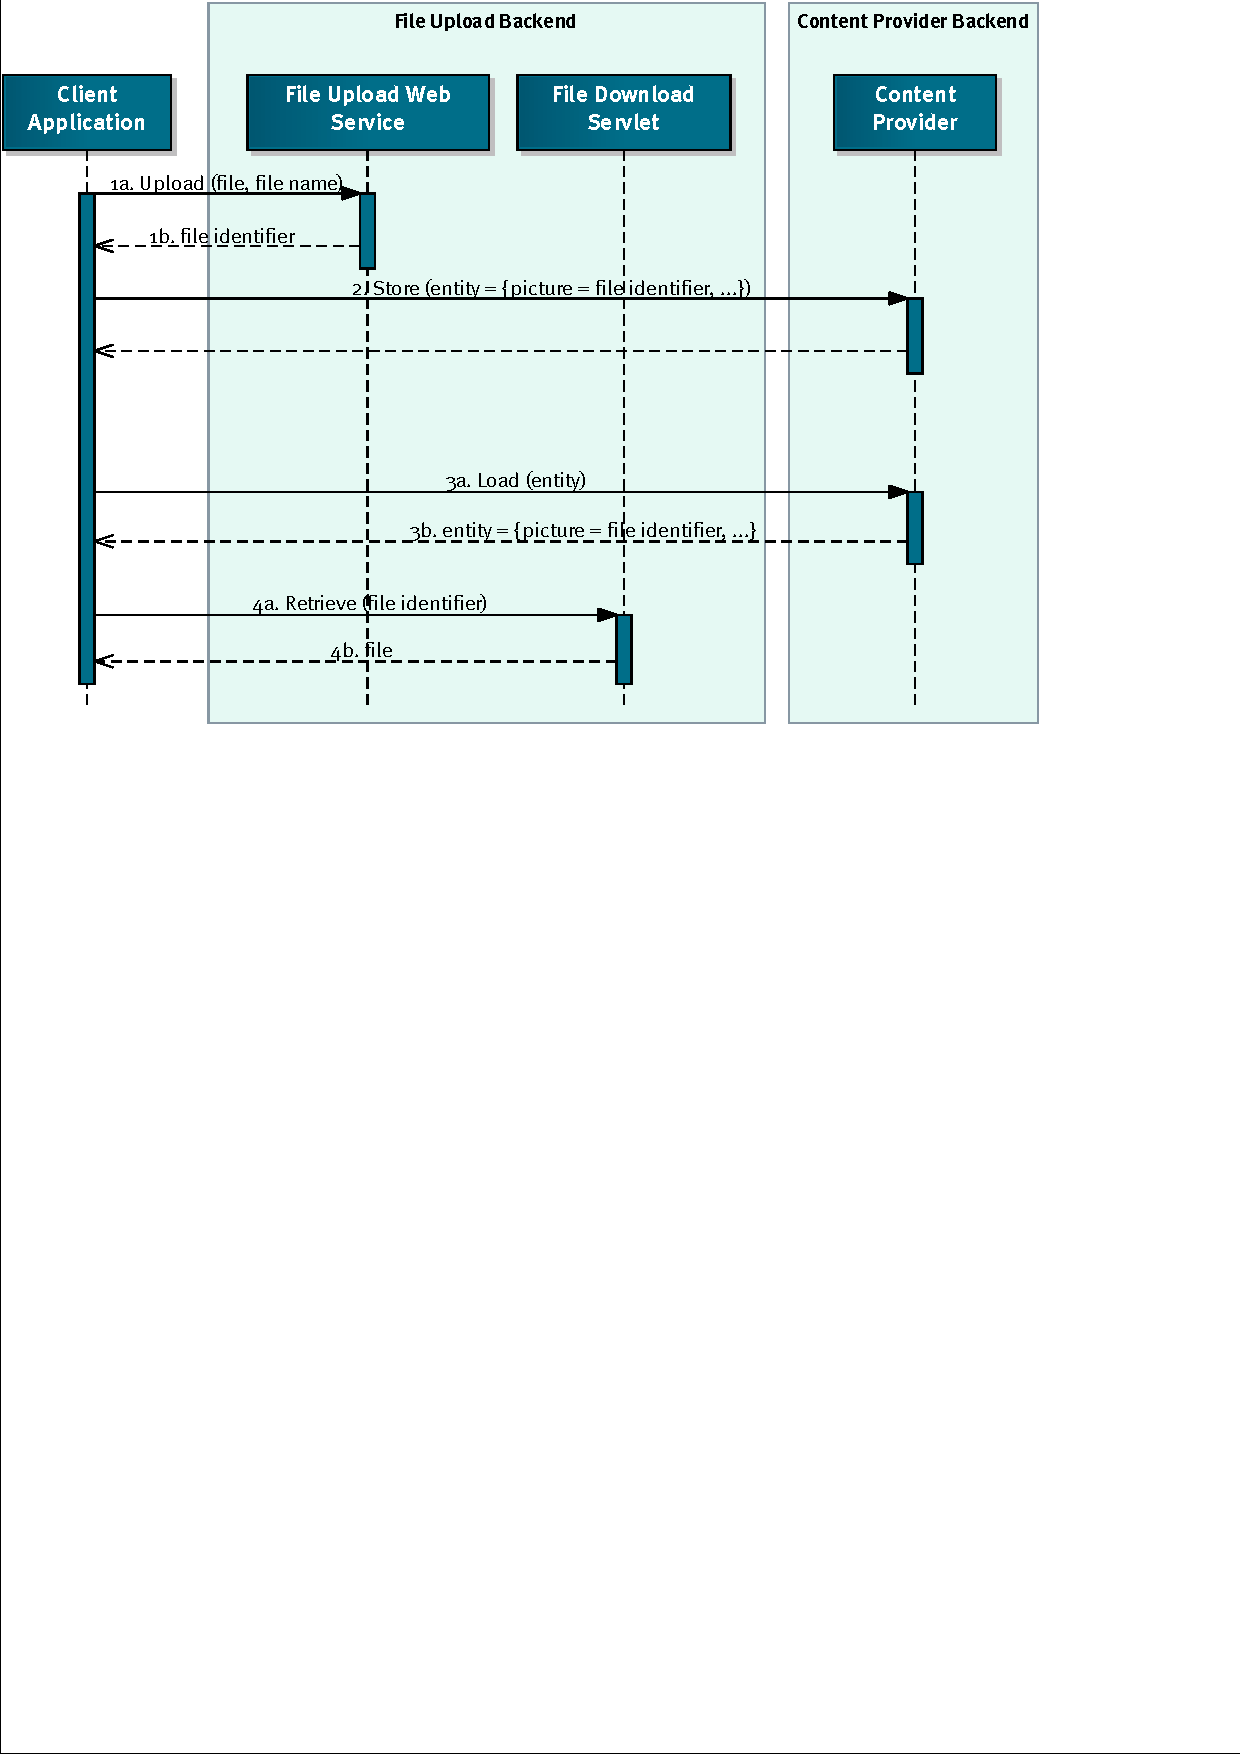
\includegraphics[width=1\textwidth, trim = 0.5mm 10cm 3.3cm 0.5mm, clip = true] {images/UML-diagrams.pdf}
\end{center}
\end{frame}

\begin{frame}[fragile]
\frametitle{Upload Images}
\codeheading{View Layer}
\begin{lstlisting}[basicstyle=\footnotesize\ttfamily]
FileUpload UploadBtn {text "Upload File"}
UploadedImageOutput imageoutput
\end{lstlisting}

\vfill

\codeheading{Controller Layer}
\begin{lstlisting}[basicstyle=\footnotesize\ttfamily]
main {
	...  
	fileUploadConnection UploadConnection
}
map MediaCapturingView.UploadBtn to :ComplaintProvider.picture
map MediaCapturingView.imageoutput to :ComplaintProvider.picture
\end{lstlisting}
\end{frame}

%-----------------------------------------------------------------------------------

%\begin{frame}
%    \frametitle{Generator}
%    
%	\begin{center}   
%	\begin{tikzpicture}[
%		>=stealth,
%		node distance = 0.75cm and 0.25cm,
%		every node/.style={minimum height = 1.75em}]
%		\node[draw] (dsl) {DSL\vphantom{Aq}};
%		\node[draw, below = of dsl] (md2model) {\MD Model\vphantom{Aq}};
%		\draw[->] (md2model) -- node[right] {\tiny{uses}} (dsl);
%	    
%		\node[below = of md2model, draw] (preprocessor) {Preprocessor\vphantom{Aq}};
%		\draw[->] (md2model) -- node[right] {\tiny{processed by}} (preprocessor);
%		
%		\node[draw, below = of preprocessor] (generator) {Generator\vphantom{Aq}};
%		
%		\draw[->] (preprocessor) -- node[right] {\tiny{input for}} (generator);
%		
%		\node[draw, below left = 0.25cm of generator] (mapapps) {map.apps source\vphantom{Aq}};
%		\node[draw, below right = 0.25cm of generator] (backend) {backend source\vphantom{Aq}};
%		
%		\draw[->] (generator) -| node[above] {\tiny{generates}} (mapapps);
%		\draw[->] (generator) -| node[above] {\tiny{generates}} (backend);
%	\end{tikzpicture}
%	\end{center}
%\end{frame}

%\begin{frame}
%    \frametitle{Deployment}
%    
%    \begin{center}   
%	    \begin{tikzpicture}[
%	    >=stealth,
%	    node distance = 0.75cm and 0.25cm,
%	    big/.style = {draw, minimum width = 2.5cm, minimum height = 1.75em}
%	    ]
%	    \node[big] (generator) {Generator};
%	    \node[big, below left = of generator] (mapapps) {map.apps source\vphantom{Aq}};
%	    \node[big, below right = of generator] (backend) {backend source\vphantom{Aq}};
%	    \draw[->] (generator) -| node[above] {\tiny{generates}} (mapapps);
%	    \draw[->] (generator) -| node[above] {\tiny{generates}} (backend);
%	    \node[big, rounded corners, below = of mapapps] (jetty) {Jetty\vphantom{Aq}};
%	    \node[big, rounded corners, below = of backend] (glassfish) {Glassfish\vphantom{Aq}};
%	    \draw[->] (mapapps) -- node[left] {\tiny{deployed on}} (jetty);
%	    \draw[->] (backend) -- node[right] {\tiny{deployed on}} (glassfish);
%	    \draw[<->] (jetty) -- node[above] (communicates) {\tiny{communicates}} (glassfish);
%	    
%	    \node[big, rounded corners, below = of communicates] (tomcat) {Tomcat};
%	    \node[big, gray, below = 0cm of tomcat] {map.apps full};	    
%	    
%	    \end{tikzpicture}
%    \end{center}
%\end{frame}

%-----------------------------------------------------------------------------------

\begin{frame}
    \frametitle{Modeling, Generation \& Deployment}
    
    \begin{center}   
	    \begin{tikzpicture}[
	    >=stealth,
	    node distance = 0.75cm and 0.25cm,
	    big/.style = {draw, minimum width = 2.5cm, minimum height = 1.75em},
	    header/.style = {big, minimum width = 3.2cm, fill=pantone315!10!white, outer sep = 0}
	    ]
	    \node[header] (eclipseDevelopment) {Framework IDE};
	    \node[big, below = 0.05cm of eclipseDevelopment] (dsl) {DSL};
	    \node[big, below = 0.05cm of dsl] (generator) {Generator};
	    
	    \node[below=1.4cm of generator, header] (generatedArtifacts) {Generated Artifacts\vphantom{Aq}};
	    \node[big, below = 0.05cm of generatedArtifacts] (backend) {Backend};
	    \node[big, below = 0.05cm of backend] (mapApps) {map.apps};
	    
	    \node[big, right = 2cm of backend, fill=pantone315!10!white] (glassfish) {Glassfish AS};
	    \node[big, right = 2cm of mapApps, fill=pantone315!10!white] (jetty) {Jetty};
	    
	    \draw[->] (backend) -- node[above] {\tiny{deploy}} (glassfish);
	    \draw[->] (mapApps) -- node[above] {\tiny{deploy}} (jetty);
	    
	    \node[header, right = 2cm of eclipseDevelopment] (eclipseModeling) {Modeling IDE};
	    \node[big, below = 0.05cm of eclipseModeling] (md2model) {\MD Model};
	    \node[below = 0cm of md2model] (modelModels) {models};
	    \node[below = 0cm of modelModels] (modelViews) {views};
	    \node[below = 0cm of modelViews] (modelController) {controllers};
	    \node[below = 0cm of modelController] (modelViews) {workflows};
	    
	    \draw[->] (md2model) -- node[above] {\tiny{uses}} (dsl);
	    \draw[->] (generator) -- node[left] {\tiny{generates}} (generatedArtifacts);
	    \draw[->] ($(eclipseModeling.south west) + (0, -1.125)$) -- node[above] {\tiny{invokes}} (generator);   

	    \draw (eclipseDevelopment.north west) rectangle ($(eclipseDevelopment.south east) + (0, -1.7)$);
	    \draw (generatedArtifacts.north west) rectangle ($(generatedArtifacts.south east) + (0, -1.7)$);
	    \draw (eclipseModeling.north west) rectangle ($(eclipseModeling.south east) + (0, -3.5)$);
	    \draw (md2model.south west) rectangle ($(md2model.south east) + (0, -2.5)$);
	    
	    
	    \end{tikzpicture}
    \end{center}
\end{frame}

    
    \section{Live Demo}
    % !TEX root = ../beamer.tex

\begin{frame}
    \frametitle{Modeling, Generation \& Deployment}
    
    \begin{center}   
	    \begin{tikzpicture}[
	    >=stealth,
	    every node/.style={outer sep = 0},
	    node distance = 0.75cm and 0.25cm,
	    big/.style = {draw, minimum width = 2.5cm, minimum height = 1.75em},
	    header/.style = {big, minimum width = 3.2cm, fill=pantone315!10!white, outer sep = 0}
	    ]
	    \node[header] (eclipseDevelopment) {Framework IDE\vphantom{Aq}};
	    \node[big, below = 0.2cm of eclipseDevelopment] (dsl) {DSL\vphantom{Aq}};
	    \node[big, below = 0.1cm of dsl] (generator) {Generator\vphantom{Aq}};
	    
	    \node[below=1.2cm of generator, header] (generatedArtifacts) {Generated Artifacts\vphantom{Aq}};
	    \node[big, below = 0.2cm of generatedArtifacts] (backend) {Backend\vphantom{Aq}};
	    \node[big, below = 0.1cm of backend] (mapApps) {\mapapps\vphantom{Aq}};
	    
	    \node[header, right = 2.3cm of backend, fill=pantone315!10!white] (glassfish) {Glassfish AS\vphantom{Aq}};
	    \node[header, right = 2.3cm of mapApps, fill=pantone315!10!white] (jetty) {Jetty};
	    
	    \draw[->] (backend) -- node[above] {\tiny{deploy}} (glassfish);
	    \draw[->] (mapApps) -- node[above] {\tiny{deploy}} (jetty);
	    
	    \node[header, right = 2cm of eclipseDevelopment] (eclipseModeling) {Modeling IDE\vphantom{Aq}};
	    \node[big, below = 0.2cm of eclipseModeling] (md2model) {\MD Model\vphantom{Aq}};
	    \node[big, below = 0cm of md2model, align=center] (modelModels) {models\\views\\controllers\\workflows};
	    
	    \draw[->] (md2model) -- node[above] {\tiny{uses}} (dsl);
	    \draw[->] (generator) -- node[left] {\tiny{generates}} (generatedArtifacts);
	    \draw[->] ($(eclipseModeling.south west) + (0, -1.3)$) -- node[above] {\tiny{invokes}} (generator);   

	    \draw (eclipseDevelopment.north west) rectangle ($(eclipseDevelopment.south east) + (0, -1.85)$);
	    \draw (generatedArtifacts.north west) rectangle ($(generatedArtifacts.south east) + (0, -1.85)$);
	    \draw (eclipseModeling.north west) rectangle ($(eclipseModeling.south east) + (0, -3.05)$);
	   % \draw (md2model.south west) rectangle ($(md2model.south east) + (0, -2.5)$);
	    
	    
	    \end{tikzpicture}
    \end{center}
\end{frame}

%-------------------------------------------------------------------------

\begin{frame}[fragile, plain]
	\plainnumber
    \frametitle{Use Case: Dating App}
    
    \begin{figure}
    	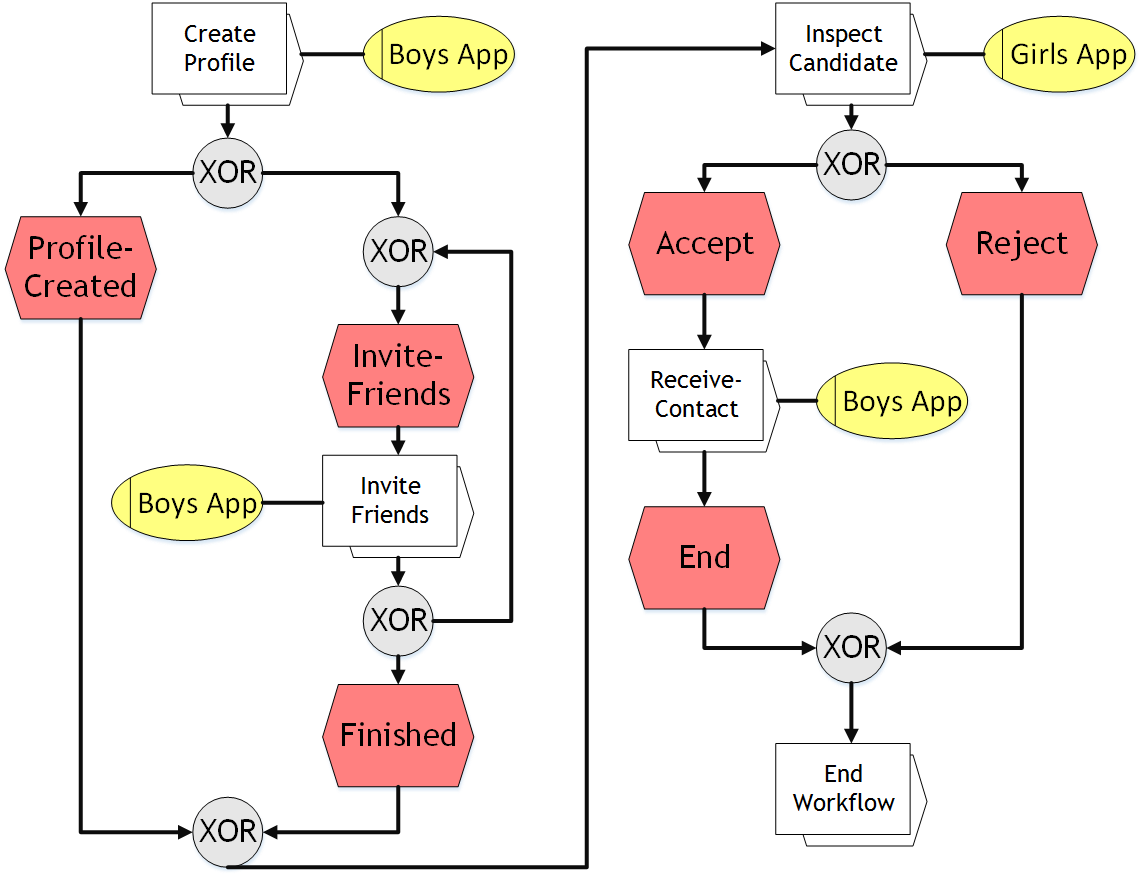
\includegraphics[width= 0.9\linewidth]{images/DatingApp.png}
    \end{figure}
\end{frame}

    
    \section[Scrum, Tests and CI]{Scrum, Tests and Continuous Integration}
    % !TEX root = ../beamer.tex
\begin{frame}
    \frametitle{Our Procedure}
    \begin{itemize}
   \item Agile software development using the Scrum methodology
   \item Scrum board with user stories and responsibilities
    \end{itemize}
    \vfill
    \begin{center}
		\begin{tikzpicture}
			\node[fill=white, draw, drop shadow] {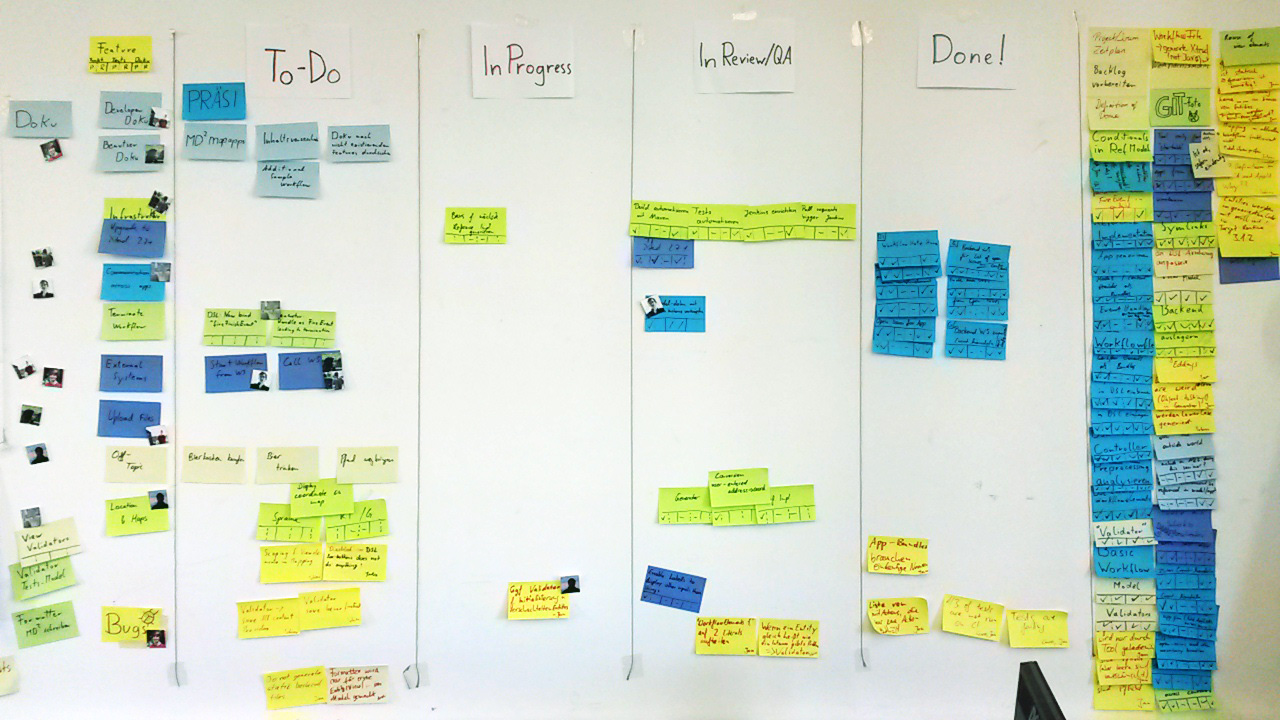
\includegraphics[height=40mm]{images/scrumboard}};
		\end{tikzpicture}
    \end{center}
\end{frame}

\begin{frame}
	\frametitle{Our Scrum Board}
    \begin{figure}
	    \begin{center}
	        \pgfimage[height=60mm]{images/scrum.png}
	    \end{center}
	\end{figure}
\end{frame}

\begin{frame}
\frametitle{Story Cards}
\begin{center}
	\begin{tikzpicture}[
		line/.style= {pantone396!50!black},
		lbl/.style= {}
	]
		\draw[fill=pantone396!10!white, draw=pantone396] (0,0) rectangle (9, 6);
		\draw[line] (0, 2) -- (9, 2);
		\foreach \x in {1.5, 4.5, 7.5}
			\draw[line, dashed] (\x, 0) -- (\x, 2);
		\foreach \x in {3, 6}
			\draw[line, ] (\x, 0) -- (\x, 2);
		
		\node[lbl] at (1.5, 2.25) {\scriptsize{Implementation\vphantom{Aq}}};
		\node[lbl] at (4.5, 2.25) {\scriptsize{Tests\vphantom{Aq}}};
		\node[lbl] at (7.5, 2.25) {\scriptsize{Documentation\vphantom{Aq}}};
		
		\node[] at (4.5, 4) {\Large{Task Description}};
		
		\node at (0.75, 1.1) {\LARGE{\textbf{\checkmark}}};
		\node at (3.75, 1.1) {\LARGE{\textbf{\checkmark}}};
		
		\foreach \x in {0.75, 3.75, 6.75}
			\node at (\x, 0.2) {\tiny{DONE}};
		\foreach \x in {2.25, 5.25, 8.25}
			\node at (\x, 0.2) {\tiny{REVIEWED}};
			
		\node[overlay, inner sep = 0, draw, rotate=6] at (7.5, 5.75) {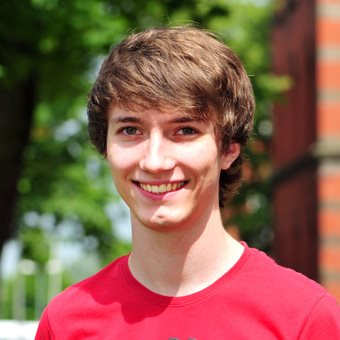
\includegraphics[width=1.75cm]{images/malte}};
		
	\end{tikzpicture}
\end{center}
\end{frame}

\begin{frame}[plain]
	\frametitle{Bugs}
    \begin{center}
		\begin{tikzpicture}
			\node[fill=white, draw, drop shadow] {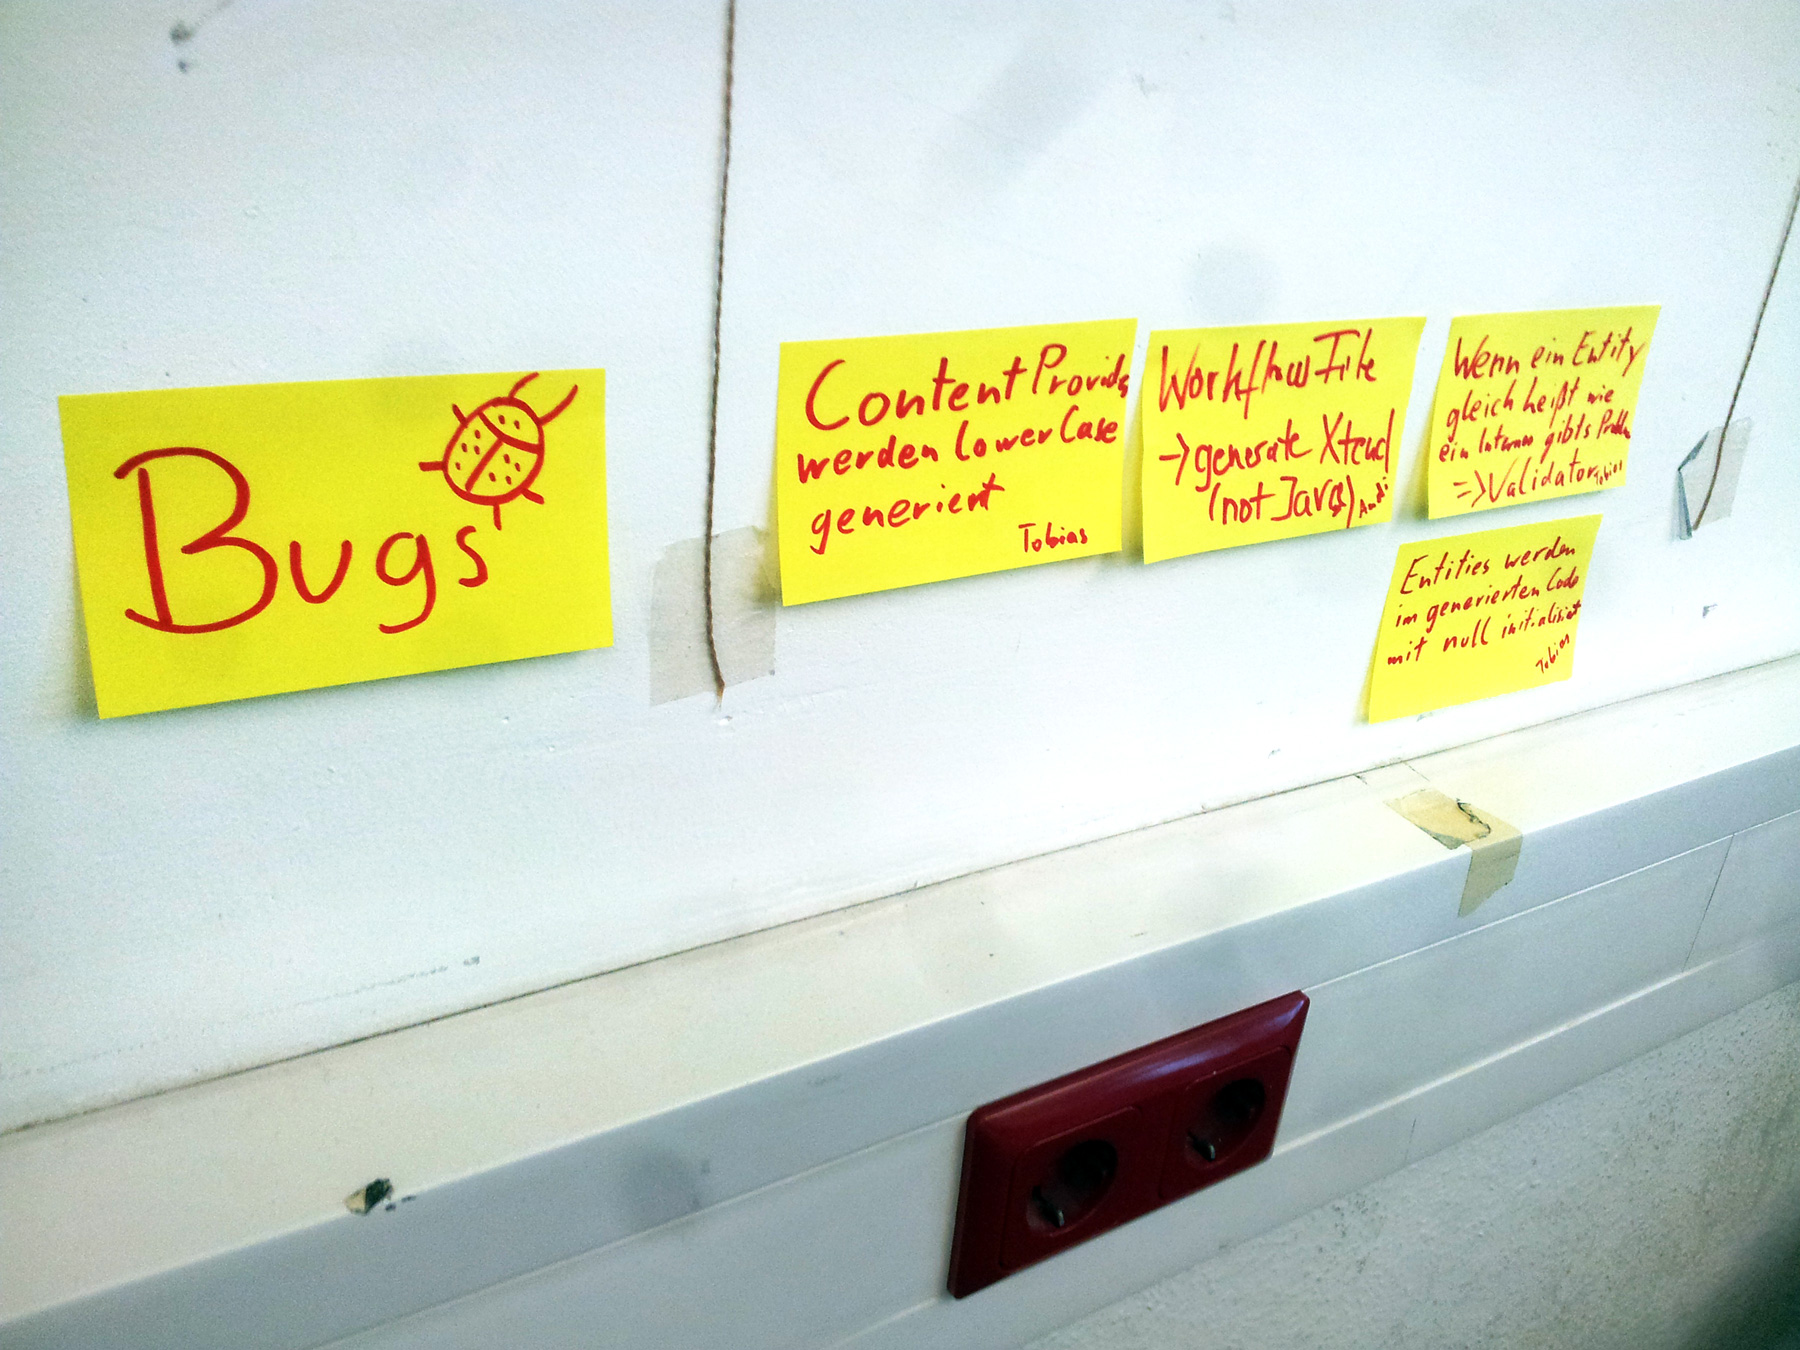
\includegraphics[width=.85\textwidth]{images/bugs}};
		\end{tikzpicture}
    \end{center}
\end{frame}


    
    \section{Conclusion}
    % !TEX root = ../beamer.tex
\begin{frame}
    \frametitle{We enhanced the DSL and generator to enable...}
    
    \begin{itemize}
    	\item Workflow specifications,
    	\item Generation of multiple apps and communication between them,
    	\item Webservice calls from within an app,
    	\item Starting workflows using a webservice,
    	\item Calculation of a punctual location from an address, and
    	\item Uploading and displaying images.
    \end{itemize}

\end{frame}

\begin{frame}
    \frametitle{Next Steps could include...}

	\begin{itemize}
		\item Adaptation of the Android and iOS generators,
		\item Renaming of workflow elements,
		\item Allowing return values for external webservice calls,
		\item Supporting temporary offline usage, and
		\item Accessing device-specific services (e.\,g., location, camera).
	\end{itemize}
\end{frame}

\begin{frame}[plain]
	\frametitle{PS-\MD in Numbers}
	\plainnumber
	\tikz[overlay]{%
		\visible<6->{%
			\draw (8.5,0.5) node[draw, fill=white, drop shadow] (img) {
\includegraphics[width=0.5\textwidth]{images/lastslide.jpg}};
			\node[below = 0.2cm of img, pantone315] {\Large{}Thank you for your attention!};
		}
	}
\begin{tabular}{r|l}~\\
	{\Large\color{pantone315} 5kg}&\visible<2->{Coffee}\\[1ex]
	{\Large\color{pantone315} 153}&\visible<2->{Coffee filters}\\[3ex]
	{\Large\color{pantone315} 300g}&\visible<3->{Loose green tea}\\[1ex]
	{\Large\color{pantone315} 50}&\visible<3->{Tea bags}\\[3ex]
	{\Large\color{pantone315} 6 pck}&\visible<4->{Post-its}\\[1ex]
	{\Large\color{pantone315} 4}&\visible<4->{Eddings}\\[1ex]
	{\Large\color{pantone315} 2}&\visible<4->{Team calendars}\\[3ex]
	{\Large\color{pantone315} A lot of}&\visible<5->{Nerves}\\[2ex] 
\end{tabular}
\end{frame}



\end{document}
